\chapter{ANÁLISE E MODELAGEM}

A primeira versão de arquitetura do projeto, será desenvolvida neste capítulo, além de
requisitos funcionais e não funcionais. Utilizarei o site "draw.io"para realizar os desenhos, fluxos
e primeira seção de arquitetura, além de exemplificar as regras da arquitetura. Nas próximas
versões do projeto, será utilizada tecnologia C4 model para exemplificar e desenhar os diagramas.

\section{Modelo Arquitetural}
Para o desenvolvimento do trabalho, utilizando modelos arquiteturais como micro ser-
viços e mensageria, será desenvolvido 5 micro serviços, todos escritos em NodeJs/NestJs e
Typescript. Para o API Gateway será desenvolvido uma aplicação em NodeJS. Como citado
anteriormente, o Gateway é o coração de uma aplicação baseada em micro serviços, para realizar
o roteamento entre eles.

Para banco de dados, será utilizado o MongoDB para salvar informações como logger
e usuários, já no Supabase, será salvo os documentos de cada usuário. Cada usuário terá uma
coleção de documentos. Foram escolhidas essas tecnologias para salvar os dados, pois são
utilizadas em larga escala em aplicações de micro serviços.

\begin{figure}[!ht]
    \centering
    \caption{Arquitetura da aplicação}
    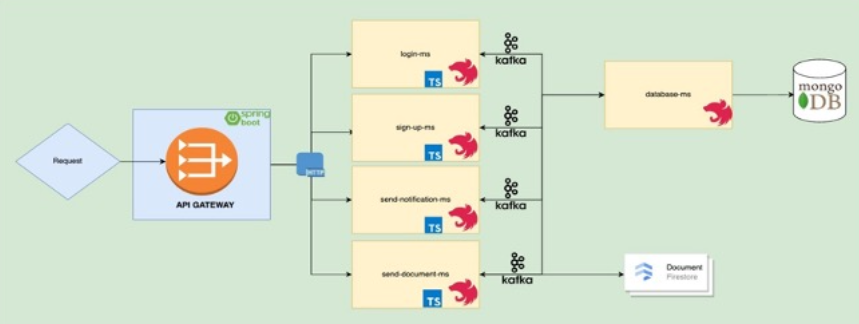
\includegraphics[scale=0.44]{assets/application-arch}
    \label{fig:application-arch}
    \tiny
    \sourcemedaddy
\end{figure}


\section{Requisitos funcionais e não funcionais}

\begin{table}[h!]
    \centering
    \begin{tabular}{|c|c|m{8cm}|}
        \hline
        \textbf{ID} & \textbf{Requisito} & \textbf{Descrição} \\ \hline
        RF-01 & Login & O usuário deve conseguir fazer login no protótipo \\ \hline
        RF-02 & Cadastro & O usuário deve conseguir se cadastrar no protótipo \\ \hline
        RF-03 & Logout & O usuário deve conseguir realizar o logout no protótipo \\ \hline
        RF-04 & Envio de documento & O usuário deve conseguir enviar documentos no protótipo \\ \hline
        RF-05 & Escolha de notificações & O usuário deve conseguir escolher quais os meios de notificação devem notificar os outros usuários \\ \hline
    \end{tabular}\label{tab:table2}
\end{table}


\section{Modelagem de Dados}

Tendo os requisitos funcionais e não funcionais, fica mais fácil definir quais dados
e quais valores serão salvos no banco de dados.
Conforme supracitado no item 3.1, para o desenvolvimento da aplicação será necessário utilizar duas tabelas, uma sendo alocada no banco
local, onde será salvo informações de notificação, e-mail, número de telefone e nome do usuário
no MongoDB, já no Supabase, será salvo as informações do identificador do usuário e todos os documentos enviados pelo mesmo.
Também haverá uma tabela de logger, para garantir que os dados sejam confiáveis, além de garantir qual era o valor do registro antigo e do registro novo.

\section{Perpectivas do Produto}

Para o protótipo, inicialmente será desenvolvido apenas uma API backend, com um
API gateway, conforme protótipo da Figura 10, além de ser desenvolvido toda a arquitetura do
protótipo em C4 utilizando ferramentas como C4 Builder.
Para trabalhos futuros, poderá ser
desenvolvido uma aplicação frontend e um aplicativo móvel para realizar o envio de documentos.

\begin{figure}[!ht]
    \centering
    \caption{Modelagem de Dados}
    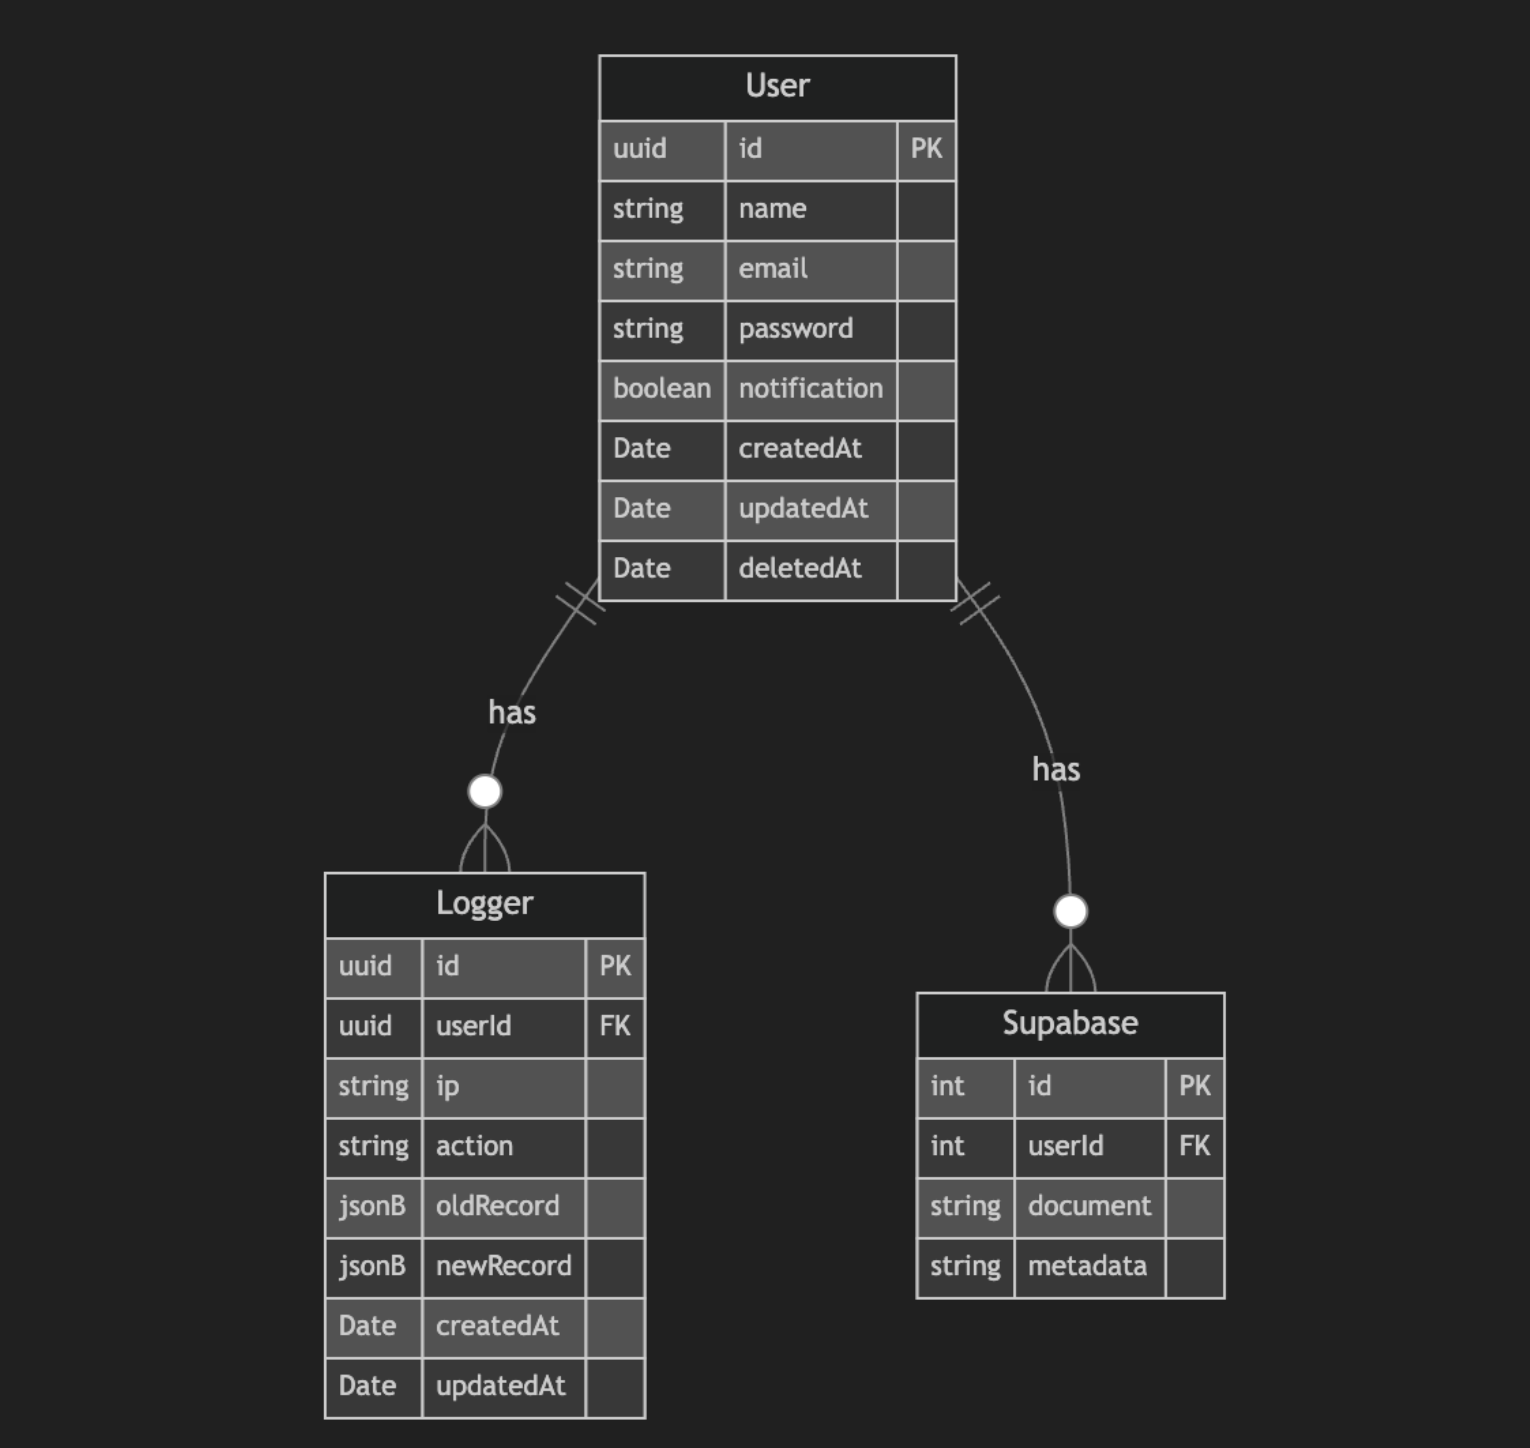
\includegraphics[scale=0.44]{assets/data-model}
    \label{fig:data-model}
    \tiny
    \sourcemedaddy
\end{figure}

O trabalho será desenvolvido localmente, e também como futuras implementações será
criado uma aplicação em nuvem.
Para envio dos documentos, será enviado para um servidor em
cloud, como o Supabase.
O Supabase foi escolhido pela facilidade de salvar os documentos em
um local criptografado.

Para projetos utilizando o Supabase, o uso de Row-Level Security (RLS) e JSON Web Tokens (JWT) é essencial para garantir um controle de acesso robusto e seguro em aplicações reais.
O RLS permite que sejam definidas regras de segurança diretamente no nível da linha de dados, garantindo que cada usuário ou grupo de usuários tenha acesso apenas aos dados autorizados, o que é essencial em sistemas multiusuário onde a privacidade e a segurança são prioritárias.
O JWT, por sua vez, possibilita a autenticação e autorização do usuário de forma segura e escalável, permitindo que o backend valide a identidade do usuário sem a necessidade de uma conexão persistente, o que é ideal para aplicações distribuídas e escaláveis.

A abordagem combinada de RLS e JWT no Supabase traz diversas vantagens para um projeto real.
O RLS oferece flexibilidade para a definição de políticas personalizadas no banco de dados, simplificando a lógica de segurança ao centralizá-la no nível dos dados.
Já o JWT facilita a integração com sistemas de autenticação modernos, permitindo a autenticação sem estado e garantindo a compatibilidade com múltiplos dispositivos e sessões.
Essa arquitetura fornece uma camada de segurança sólida e facilmente escalável, essencial para o desenvolvimento de aplicativos seguros e eficientes, otimizando tanto a experiência do usuário quanto a segurança dos dados.





